\documentclass{bioinfo}
\usepackage{booktabs}
\copyrightyear{2015} \pubyear{2015}

\access{Advance Access Publication Date: Day Month Year}
\appnotes{Manuscript Category}

\begin{document}
\firstpage{1}

\subtitle{Subject Section}

\title[short Title]{Pseudo batch transformation: A method to correct for mass removal through sample withdrawal of fed-batch fermentation}
\author[Sample \textit{et~al}.]{Corresponding Author\,$^{\text{\sfb 1,}*}$, Co-Author\,$^{\text{\sfb 2}}$ and Co-Author\,$^{\text{\sfb 2,}*}$}
\address{$^{\text{\sf 1}}$Department, Institution, City, Post Code, Country and \\
$^{\text{\sf 2}}$Department, Institution, City, Post Code,
Country.}

\corresp{$^\ast$To whom correspondence should be addressed.}

\history{Received on XXXXX; revised on XXXXX; accepted on XXXXX}

\editor{Associate Editor: XXXXXXX}

\abstract{\textbf{Motivation:} Text Text Text Text Text Text Text Text Text Text Text Text Text
Text Text Text Text Text Text Text Text Text Text Text Text Text Text Text Text Text Text Text
Text Text Text Text Text Text Text Text Text Text Text Text Text Text Text Text Text Text Text
Text Text Text Text Text Text
Text Text Text Text Text.\\
\textbf{Results:} Text  Text Text Text Text Text Text Text Text Text  Text Text Text Text Text
Text Text Text Text Text Text Text Text Text Text Text Text Text  Text Text Text Text Text Text\\
\textbf{Availability:} Text  Text Text Text Text Text Text Text Text Text  Text Text Text Text
Text Text Text Text Text Text Text Text Text Text Text Text Text Text  Text\\
\textbf{Contact:} \href{name@bio.com}{name@bio.com}\\
\textbf{Supplementary information:} Supplementary data are available at \textit{Bioinformatics}
online.}

\maketitle

\section{Introduction}
% fed-batch is popular for industry
Fed-batch cultivation methods are popular in the Biomanufactoring industry because they typically enable high cell densities and titers. For production strains which suffer from substrate inhibition or overflow metabolism fed-batch processes can increase productivity and are simpler to operate compared with continuous fermentation processes \citep{ramirezExponentiallyFedbatchCultures1994,mearsReviewControlStrategies2017}.

% provides XX good process characteristics 
Unfortunately, analysing fed-batch data is non-trivial due to the volume changes of the bioreactor. Due to these changes, mass balances must be resolved on the basis of mass instead of concentration. When samples are withdrawn from the bioreactor mass is removed from the system. This results in discontinuous mass time-evolution curves. This discontinuous behaviour requires special attention when researchers subsequently estimate rates and yields.

The discontinuous jumps become larger when the sample-to-reactor-volume ratio increase. This is particularly pronounced in miniaturised fermentation systems such as Satorious' AMBR or Beckmann's Robolector, but the sample-to-reactor-volume ratio can also become large for non-miniaturised setups where significant samples are withdrawn in order to prevent the reactor from filling up or prolong the cultivation time.

In this study, we present a transformation method called pseudo batch transformation, which removes the effects of volume changes from the data. The pseudo batch transformed data is the equivalent batch fermentation data, if it were possible to add feed without volume changes. Using simulated data, we show that the correct rates and yields can be estimated from the transformed data using standard methods, such as linear models.

The pseudo batch fermentation is available as a python package and as an excel-sheet, where the user can input their own data.




%\enlargethispage{12pt}

\section{Approach}

Equation~(\ref{eq:01}) Text Text Text Text Text Text  Text Text
Text Text Text Text Text Text Text Text Text Text Text Text Text.
Figure~2\vphantom{\ref{fig:02}} shows that the above method  Text
Text Text Text  Text Text Text Text Text Text  Text Text.
\citealp{Boffelli03} might want to know about text text text text
.....


\begin{methods}
\section{Methods}
\subsection{Pseudo batch transformation}
\begin{equation}\label{eq:transformation}
c^{\star}_{species,\: k} = ADF_k \cdot c_{species, \: k} - \sum_{j=1}^{nf} \sum_{i=1}^{k}ADF_i\frac{c_{species, \: feed_{j}} \cdot F_{i,j}}{V_i}
\end{equation}
\begin{itemize}
    \item $c^{\star}_{species,\: k}$ is the pseudo concentration
    \item $V_i$ is the before sample volume at time $i$
    \item $c_{species, \: feed_{j}}$ is the concentration of the species in the feed $j$
    \item $F_i$ is the feed during the measurement past interval
    \item $ADF_k$ is the accumulated dilution factor $ADF_k = \prod_1^k\frac{V_k}{V_{k-1} - S_{k-1}}$, where $S$ is the sample volume, which is 0 at time points where no sample was withdrawn.
    \item $nf$ is the total number of feed medium
\end{itemize}


\subsection{Simulated data}
To validate the pseudo-batch transformation method, we created a set of Julia \cite{bezansonJuliaFreshApproach2017} and Python \cite{rossumPythonLanguageReference2010} scripts that simulate the growth of an organism in a fed-batch process. The simulated microbial culture consumes glucose and produces biomass, a generic product and $CO_2$ according to the following system of ordinary differential equations:
\begin{align} % NB these equations are lack some editing
\frac{dm_{s}}{dt} &= -Yxs * mu(m_{s}) * m_{x} \\ &+ v_{feed}(t, F0, mu0) * c_f \\
\frac{dm_{x}}{dt} &= mu(m_{s}) * m_{x} \\
\frac{dm_{p}}{dt} &= Yxp * mu(m_{s}) * m_{x} \\
\frac{dm_{co2}}{dt} &= Yxco2 * mu(m_{s}) * m_{x} \\
\frac{dV}{dt} &= v_{feed}(t, F_0, \mu_0)
\end{align}
Where Yxs, Yxp, and Yxco2 are the biomass yield coefficients, in $\frac{g}{g}$, of glucose, a generic product and CO2; $m_{s}$, $m_{p}$, and $m_{co2}$ are the mass in grams of glucose, a generic product, and $CO_2$, respectively; $c_f$ is the concentration of glucose in the feed medium and $v_{feed}(t)$ is the feeding profile, i.e. the flow rate of the feed medium at time $t$. 

The growth rate was modelled through one of two different functions, either using non-inhibited Monod's equation \ref{eq:monod_eq} or a product inhibition equation \ref{eq:monod_prod_inhib_eq}:
\begin{align}
\mu(t) &= \mu_{max}\frac{c_{s}(t)}{c_{s}(t) + K_{s}} m\label{eq:monod_eq} \\ 
\mu(t) &= \mu_{max}\frac{c_{s}(t)}{c_{s}(t) + K_{s}}\frac{c_{p}}{c_{p} + K_{i}} \label{eq:monod_prod_inhib_eq}
\end{align} 
The feeding profile is calculated to achieve a constant specific growth rate through the following equation:
\begin{align}
v_{feed}(t, F_0, \mu_0) = F_0 * e^{\mu_0 t}
\end{align}

To simplify the testing and validation, we used the exact values for Ysx and X0 when calculating the feeding profile, even though these would not be exactly known in a true experimental setup.

We simulated samples of the fed-batch process using callbacks that were activated at specific time points. A given volume was removed from the simulated bioreactor, and with that also mass of the species in the culture. The feeding profile was then adjusted to accommodate the decrease in total biomass. This adjustment was required to maintain a constant specific growth rate. The adjusted feeding profile was calculated as follows:
\begin{align}
    F_{0}^{adjusted} &= F_{0}^{original} * \frac{V_{after \: sampling}}{V_{before \: sampling}} \\
    v_{feed}^{adjusted}(t) &= F_{0}^{adjusted} * e^{\mu_0 t}
\end{align}
    
The growth parameters were set to textbook estimates for \textit{Saccharomyces cerevisiae}. Their exact values can be found in the supplementary content table XX. To avoid an initial adaptation phase in the growth rate, we calculated the glucose concentration resulting in the desired growth rate by isolating $\mu$ in equation \ref{eq:monod_eq}.

\subsection{Estimation of overall rates and yields}
We estimated the overall growth rate over the entire simulation period using a log-linear model in which the log-transformed biomass in either mass or concentration is a linear function of time.
\begin{align}
    log(c^{\star}_x(t)) &= a + \mu \cdot t \\
    log(m_x(t)) &= a + \mu \cdot t    
\end{align}

where $c^{\star}_x(t)$ is the pseudo biomass concentration and $m_x(t)$ is the non-corrected mass at measurement at time $t$, and $\mu$ is the fitted specific growth rate.

The overall yield coefficients, e.g. $Y_{sx}$, were estimated as the slope of a linear model between the measurements of the two species. (TEDDY: reference?) For comparison we also formulated the following two linear models for the non-corrected data: 
\begin{align}
    cm_s(t) &= b + Y_{xs} \cdot m_x(t) \\
    m_p(t) &= b + Y_{xp} \cdot m_x(t) \\
\end{align}
where $cm_s(t)$ is the consumed mass of substrate at time $t$, calculated as $cm_s(t) = m_s(0) + \int_0^t v_{feed}(t) * c_f - m_s(t)$. The following two models were used to estimate overall yield coefficients from pseudo batch transformed data.
\begin{align}
    cc^{\star}_s(t) &= b + Y_{xs} \cdot c^{\star}_x(t) \\
    c^{\star}_p(t) &= b + Y_{xp} \cdot c^{\star}_x(t) \\
\end{align}
where $cc^{\star}_s(t)$ is the consumed pseudo concentration of substrate at time $t$, calculated as $cc^{\star}_s(t) = c^{\star}_s(0)- c^{\star}_s(t)$. The parameter estimates of the all linear models were obtained as the least-squares solution.


\end{methods}

%\begin{figure}[]%figure1
%\centerline{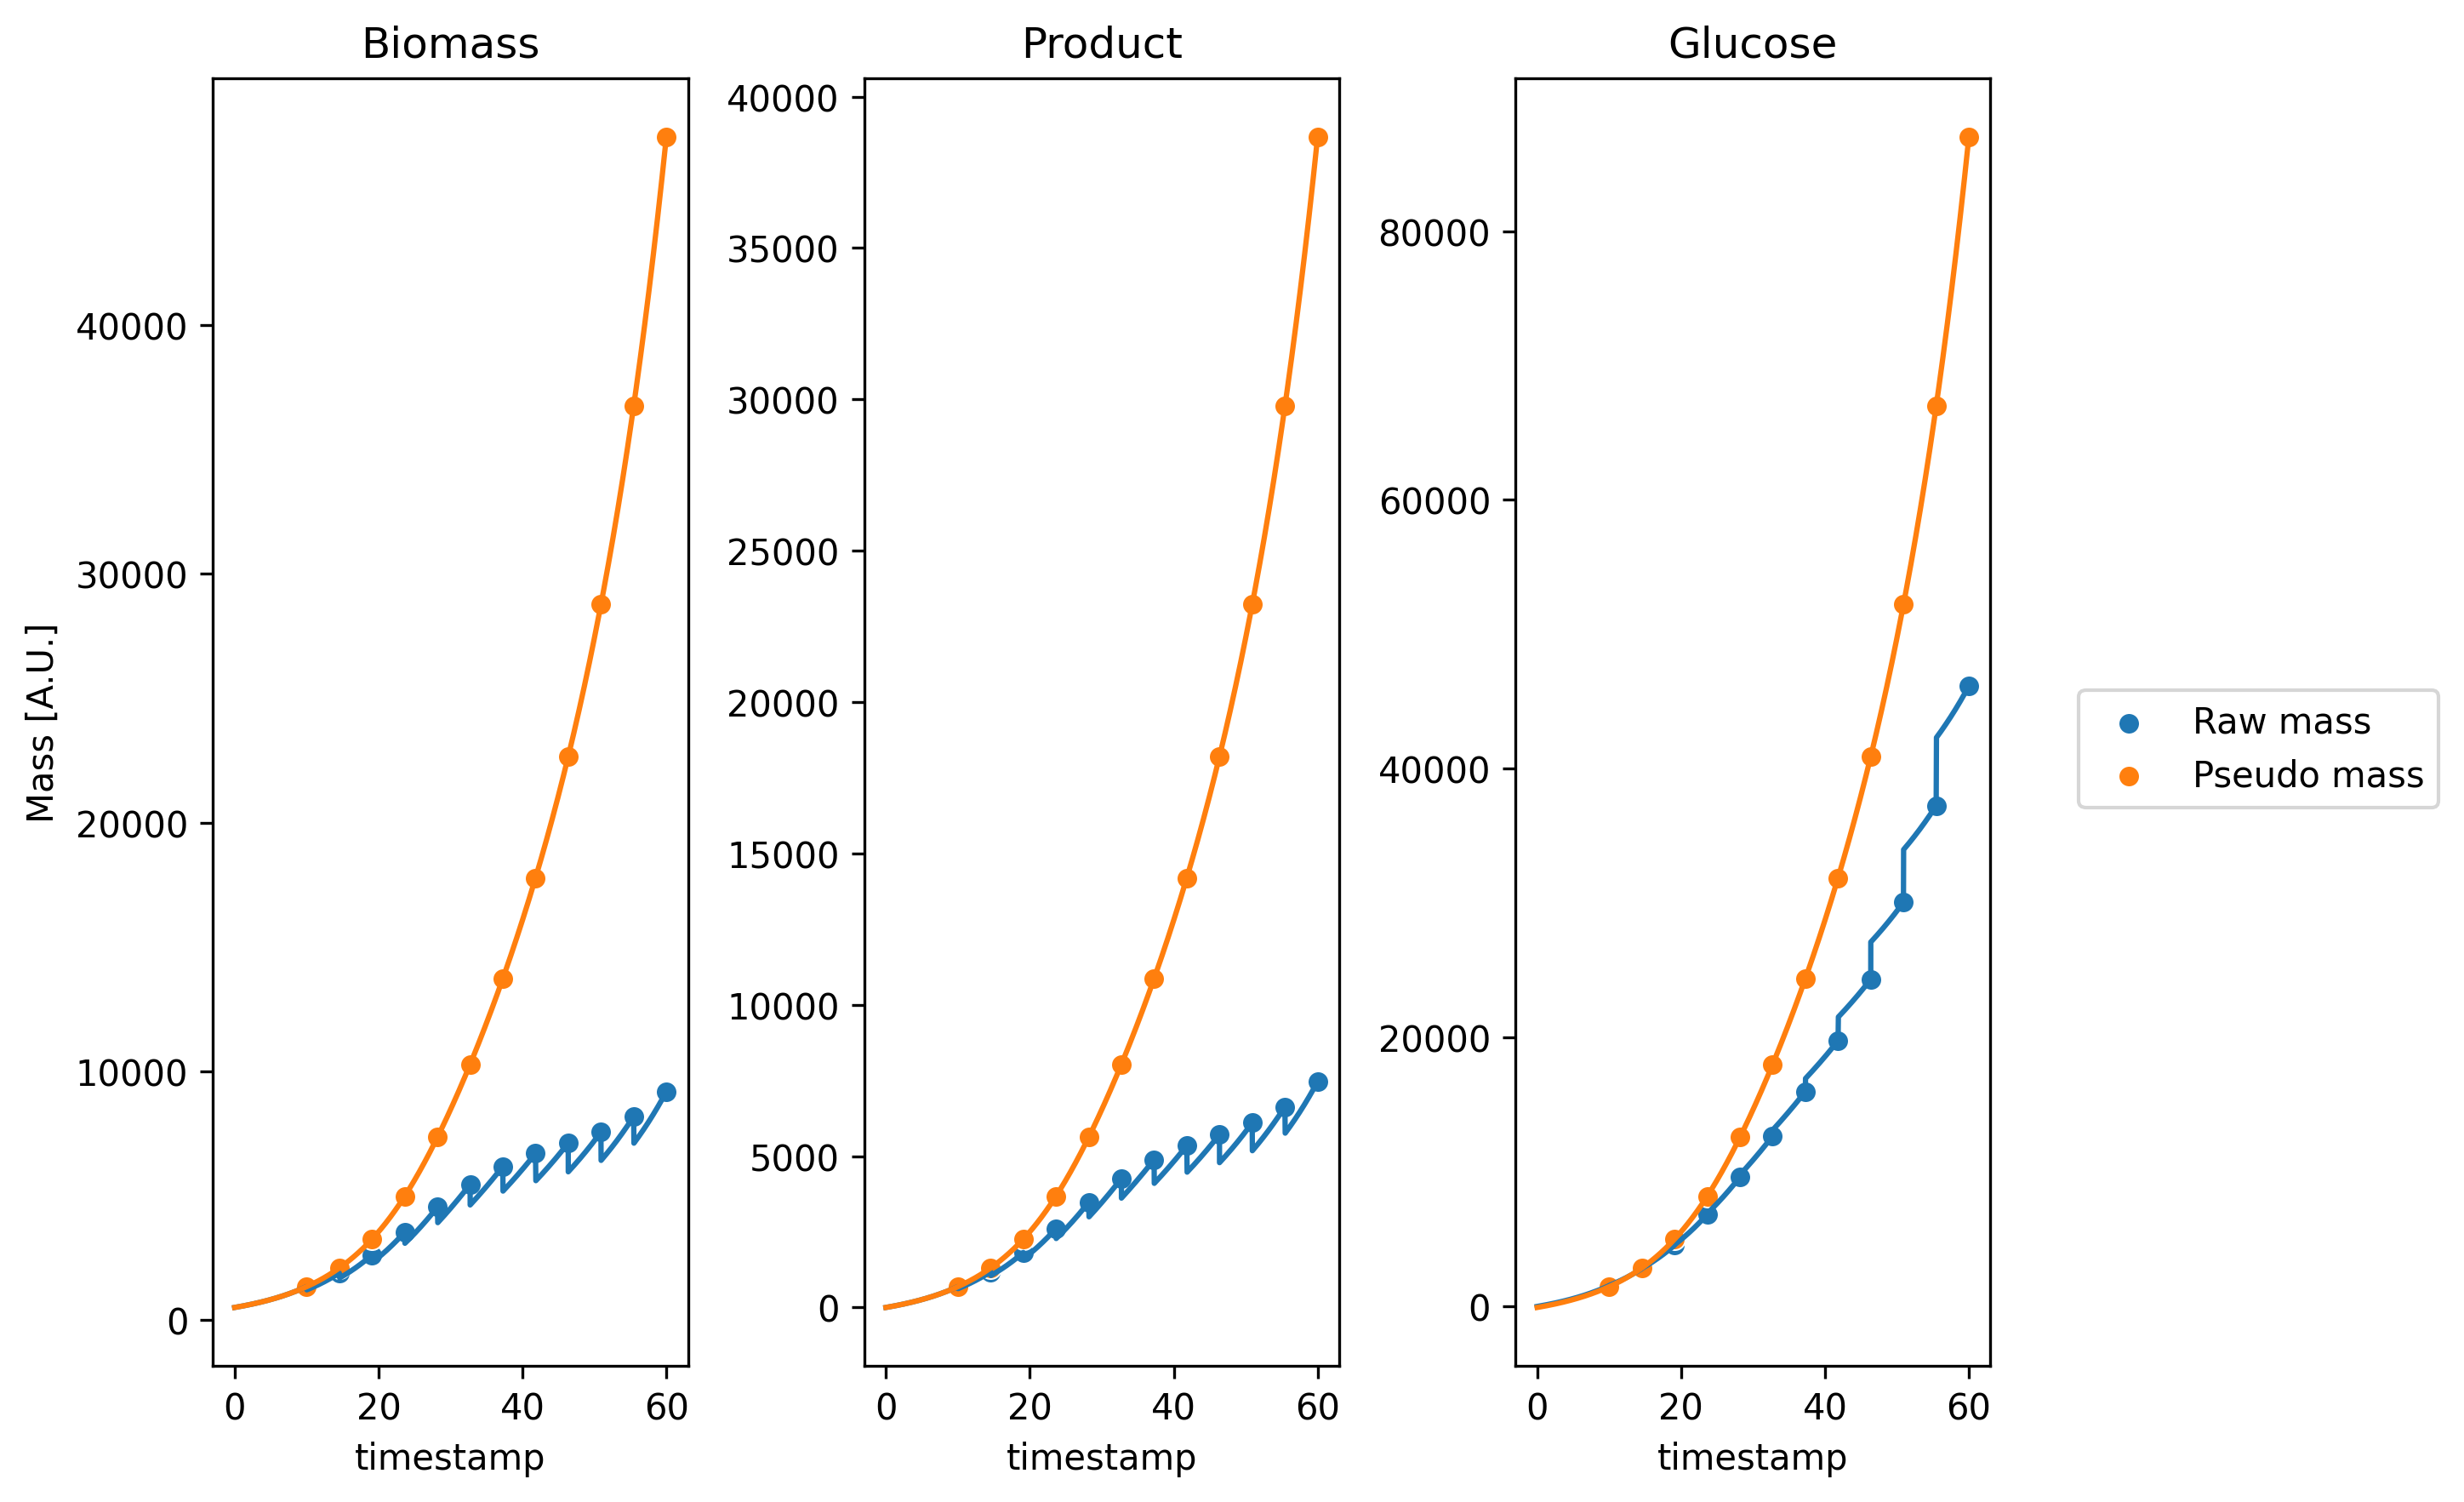
\includegraphics{figures/mass_time_course_product_inhibit.png}}
%\caption{Caption, caption.}\label{fig:mass_time_course}
%\end{figure}

%\begin{figure}[!tpb]%figure2
%%\centerline{\includegraphics{fig02.eps}}
%\caption{Caption, caption.}\label{fig:02}
%\end{figure}

\subsection{Bayesian model}
Permanent bias in feed
$y_F \sim LN(log(F * \alpha), \sigma_F)$

\section{Results and dicussion}

\subsection{Why is pseudo batch transformation necessary}
The simplest visualization of the issue is a fed-batch cultivation operated with an exponential feeding profile set up to keep the substrate concentration constant. When samples are withdrawn from this culture, mass is removed and the true underlying mass time course becomes discontinuous (Figure \ref{fig:pseudo_batch_growth_rate} - grey line). Thus, if we try to estimate the growth rate from this data using a log-linear model, we obtain a wrong value (Figure \ref{fig:pseudo_batch_growth_rate} - blue line). If we apply the pseudo-batch transformation to the data before estimating the growth rate, we obtain the correct values (Figure \ref{fig:pseudo_batch_growth_rate} - orange line). The same issue applies to the substrate and product yields, which is also wrongly estimated if special care is not taken (Table \ref{tab:compare_estimates}). 

Handling data from fed-batch fermentations can complicated, especially for mammalian cell cultures, which utilizes multiple feeding mediums and feeding profiles customized each reactor (Ref. to some of CHO-groups papers). The pseudo batch transformation handles such setups as well for more information see the documentation (LINK to tutorial - multiple feeds).

\begin{figure}
    \centering
    
\includegraphics[width = 0.4 \textwidth]{figures/transformed_and_non-transformed_logscale_paper.png}
    \caption{Caption}
    \label{fig:pseudo_batch_growth_rate}
\end{figure}

\begin{table}
    \caption{Show the true and estimated values of the yields and growth rate.}
    \label{tab:compare_estimates}
    \begin{tabular}{lccc}
     & True & Non-corrected (rel. error \%) & Corrected (rel. error \%) \\
    Yxs & 1.85 & 2.69 (-0.45) & 1.85 (0.00) \\
    Yxp & 0.82 & 0.83 (-0.01) & 0.82 (-0.00) \\
    Yxco2 & 0.05 & 0.05 (-0.01) & 0.05 (-0.00) \\
    mu & 0.10 & 0.07 (0.34) & 0.10 (-0.00) \\
    \end{tabular}
\end{table}

\subsection{The pseudo batch equation}
The pseudo batch transformation transforms the measurements into what we call the pseudo-transform space. In this space, the volume is constant, thus mass is removed or added without a change in volume. The transformed measurements should not be interpreted as an actual prediction of the theoretical fed-batch without volume change. Rather the transformation removes the effect of the volume change to ease the interpretation and data processing of the measurements. 

The pseudo batch transformation equation (equation \ref{eq:transformation} above) contains two terms: $ADF_k \cdot c_{species, \: k}$ and $- \sum_{i=1}^{k}ADF_i\frac{c_{species, \: feed} \cdot F_{i}}{V_i}$. The first term accounts for the addition or removal of volume by scaling the concentration with the accumulated dilution factor (ADF). The dilution factor is the ratio between the current volume just before sampling and the previous time point just after sampling. The dilution factor is always above one and the accumulated dilution factor will keep increasing. Thus, this term simply increases the concentration with the amount that it was diluted - cancelling out the effect of the dilution. The second term deals with the addition of mass to the bioreactor through feeding. The mass is also scaled with the ADF, thus the overall mass fed in the pseudo batch process is larger than in the real process. This term is only relevant for species that are fed and thus is zero for species that are not present in any of the feed mediums.

%This phenomenon does not only applies to exponential fed-batch cultivations. When the volume of the bioreactor changes due to feeding calculations of rates and yields must be done on a mass basis, but this becomes difficult when the true underlying time course is discontinuous. We see that discontinuous mass time course is problematic in a constant feed (Figure XX) and impulse feed fed-batch cultivations (Figure XX).

%\subsection{Relationship between error and sample volume}
%We hypothesised that the main factor which influences the estimation error made, when not accounting for mass loss, is the sample volume fraction. Using the simple exponential fed-batch with varying sample sizes, we found the estimation increases drastically when the sample size increases, for example, XX \% estimation error for 5\% sample volume fractions and XX \% at 30 \% sample volume fractions (Figure XX). A Morris sensitivity analysis showed that the magnitude of these errors depends on the specific parameters for the simulation, though for the growth rate, the error was more than 4.4\% in 95\% of the simulations (Supplementary content).

%\subsection{Pseudo batch transformation enables better rate estimates}
%A common goal for data analysis of fed-batch processes is to estimate the production or consumption rates over time, for example, to identify if the production rate changes at some point during the cultivation. Thus instead of determining one rate for the full culture, the aim is to calculate the rate at each measurement point. There are many methods to do this, but the simplest is the finite difference method. The simplest finite difference method is the first order difference $\frac{dm_i}{dt} \approx \frac{m_i(t_k)-m_i(t_{k-1})}{t_k - t_{k-1}}$. One can apply this method to the raw data by calculating how much product was produced between two samples, $\frac{dm_i}{dt} \approx \frac{m^{after}_i(t_k)-m^{before}_i(t_{k-1})}{t_k - t_{k-1}}$. When we used this method to calculate both the specific and volumetric rates, the estimated rates were consistently biased, underestimating the rate (Figure XX). These estimates only take into account two data points at a time. The pseudo batch transformed data allows us to use higher-order finite difference estimates and, in that way, including more data points when estimating the rates. This results in more accurate and unbiased estimates (Figure XX). Furthermore, the pseudo-batch transformed data allows researchers all sorts of data smoothing, outlier detection or other algorithms that utilise more than two data points simultaneously. We believe that this will enable a many interesting analysis of fed-batch data. 

%We hypothesised that using higher-order finite difference methods to estimate the specific and volumetric rates would decrease the effect of measurement error. Surprisingly, we did not observe a reduction in the variance of the relative error when using higher-order finite difference methods. This could be explained by introducing noise when the rate estimate is divided by the noisy biomass measurement when calculating specific growth rates.

\subsection{Benefits of the pseudo batch transformation}
A common procedure in the analysis of biological cultivation data is to segment the growth curve into growth phases; for which duration do the cells grow exponentially and does the growth rate appear to change at some point? This can be done through visual inspection of time series data plots, but it is difficult when the removal of mass through sampling is not corrected in the plot. 

Additionally, many statistical modelling frameworks for growth data cannot work with the discontinuous data obtained from a sampled fed-batch cultivation (Reference some examples). As we showed earlier the simple log-linear model fails to estimate the growth rate. The pseudo batch transformed data can be used in the standard linear model workflows in Excel, R or Python. Furthermore, the continuous nature of the pseudo batch transformed data enables a big suite of more advanced statistical methods to work straight out of the box. For example, one can utilise gaussian process regression to estimate the rates as a function of time with uncertainty estimation (ref: guassian process growth rate paper). Additionally, the pseudo batch transformed data greatly simplifies the analysis of data from fed batch cultivations using statistical models involving splines, dynamic flux balance analysis, and ordinary differential equation models.

\subsection{Real data}
To show the pseudo-batch transformation on some real data, we used a fed-batch cultivation data set from an earlier study (MISSING ref. to systems biology article). This data set contains 8 growth curves of \textit{S. cerevisiae}. For a duration of 33 hours of feeding two of the cultures are not sampled, two cultures are sampled twice, and four cultures are sampled once. When the pseudo batch transformation is applied to the online biomass measurements of the sampled cultures becomes continues and follows the non-sampled cultures. Note how the growth rate seems to increase after a culture is sampled, this is because the feeding is not adjusted for mass removal resulting in overfeeding and an increased growth rate. In our opinion, this example illustrates how the pseudo batch transformed data is easier to interpret visually compared with raw data.

\ref{fig:real_data}).

\begin{figure}
    \centering
    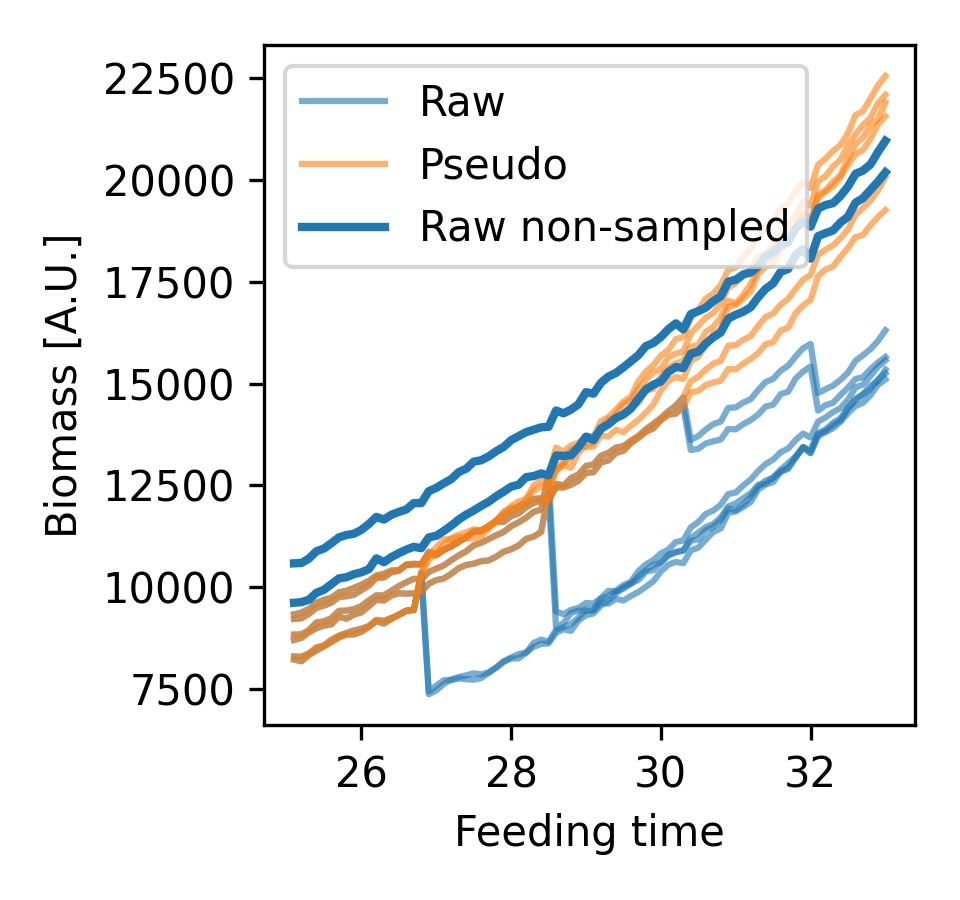
\includegraphics[width = 0.4 \textwidth]{figures/real-data-compare-paper.png}
    \caption{Caption}
    \label{fig:real_data}
\end{figure}

\subsection{Error propagation through the pseudo batch transformation}
The pseudo-batch transformation utilizes a cumulative product operation to calculate the accumulated dilution factor. We were concerned that this operation would inflate the uncertainty of the pseudo-batch concentrations. Therefore, we implemented the pseudo batch transformation in a generative Bayesian model. With this model, we investigated how the measurement error propagates through the pseudo-batch transformation. Our analysis revealed that if the concentration measurements have a coefficient of variance of 5\% (equivalent to 95\% measurement uncertainty of ±10\%), then the pseudo batch concentration has a coefficient of variance of approximately 5.02\%. This minor increase in coefficient of variation is likely caused by the uncertainty of the other modelled quantities, such as reactor volume and sample volume. In conclusion, the pseudo batch transformation does not dramatically increase the coefficient of variation of the concentration values.

\section{Conclusion}


\section*{Acknowledgements}

Text Text Text Text Text Text  Text Text.  \citealp{Boffelli03} might want to know about  text
text text text\vspace*{-12pt}

\section*{Funding}

This work has been supported by the... Text Text  Text Text.\vspace*{-12pt}

\bibliographystyle{natbib}
\bibliography{references}

\end{document}
